Un problema molto conosciuto e diffuso nelle letteratura relativa al reinforcement learning (RL) è quello del bilanciamento del  \textit{Cart Pole}.

Esso non è altro che una semplice asta collegata ad un carrello tramite un joint non attuato : questo significa che l'asta risulta essere libera di muoversi, per il semplice fatto che non vi è applicata alcuna azione esterna, proprio come un pendolo inverso.

Come si può ben capire dall'immagine in figura ~\ref{fig:CartPole}, il Cart Pole rappresenta un sistema instabile: infatti, senza un aiuto esterno, il pendolo cadrebbe verso la posizione verticale, spostandosi nell'altro equilibrio stabile (ovvero quello ovvio).

\begin{figure}[h]
	\centering
	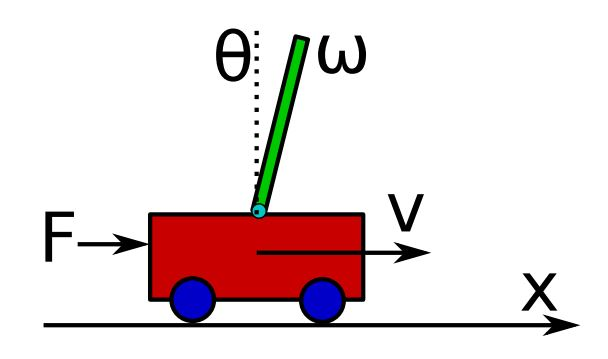
\includegraphics[width=0.5\textwidth]{Immagini/CartPole.JPG}
	\caption{Cart pole e variabili di stato}
	\label{fig:CartPole}
\end{figure}

La risoluzione di questo problema di equilibro verte sull'ambito della \textit{dinamica} e della \textit{teoria del controllo} ed è spesso utilizzato come \textit{problema dummy} per verificare e testare alcune strategie.

Si capisce quindi che, per mantenere il pendolo inverso nella posizione di equilibrio instabile, risulta essere necessario andare ad applicare una coppia sul punto di giunzione tra l'asta e il carrello, andando a muovere orizzontalmente a destra e a sinistra il carrello stesso.